\section{Numerical representation and its control}
\label{app:numerics}
\paragraph{The recursion.}
The two message sweeps of \cref{sec:setup} are
\begin{equation}
\begin{aligned}
  \lmsg_i(a)&\propto\!\int\!\kernel(a\mid a')\,\like(x_{i-1}\mid a')\,\lmsg_{i-1}(a')\dd a',\\
  \rmsg_i(a)&\propto\!\int\!\kernel(a''\mid a)\,\like(x_{i+1}\mid a'')\,\rmsg_{i+1}(a'')\dd a'',
\end{aligned}
\label{eq:bp}
\end{equation}
with $\lmsg_1\equiv\mu$, the initial law, and $\rmsg_{\nsites}\equiv1$; the site marginal is $\propto\lmsg_i\like\rmsg_i$
and Tweedie's identity turns its mean into the score.



Messages are represented on a uniform grid of $\ngrid$ points on
$[-\halfwidth,\halfwidth]$ with composite trapezoidal weights; the recursion is a scaled
linear-domain forward--backward whose discarded constants are accumulated so the
evidence $\log\Pt(\vx)$ of the discretised model is exact to floating point. Three
levels of exactness are kept apart: sum-product is exact at the level of functional
messages; forward--backward is exact for the discretised factor model; and that model
approximates the continuous chain with truncation (mass outside $[-\halfwidth,\halfwidth]$)
and quadrature (second order in the spacing) errors that are measured, not assumed.

\paragraph{Validation where the answer is known.}
\begin{proposition}[The Gaussian chain: score, smoother and sum-product coincide]
\label{prop:kalman}
Let the driving noise of \cref{eq:prior} be Gaussian, so that $\va\sim\normal{0}{\Sig_0}$ with
$(\Sig_0)_{ij}=\corr^{|i-j|}$, and let $\vx$ follow \cref{eq:channel}. Then
(i) $\score(\vx,t)=-\Sig_t^{-1}\vx$ and $\pmean{\va}=e^{-t}\Sig_0\Sig_t^{-1}\vx$, with
$\Sig_t=e^{-2t}\Sig_0+\Dt\Id$, and Tweedie's identity holds between them; (ii) every message of
\cref{eq:bp} is Gaussian, $\lmsg_i$ is the Kalman filter's prediction density
$p(a_i\mid x_{1:i-1})$ and $\lmsg_i\like$ its filtering density, and the site marginals
$\propto\lmsg_i\like\rmsg_i$ are those of the Rauch--Tung--Striebel smoother, whose means are
therefore $\pmean{\va}$ of (i).
\end{proposition}
The proof is in \cref{app:proofs}; \cref{fig:gaussian} measures it (\textsc{e39}). An RTS
smoother written without the BP code (\codefile{src/markov\_score/kalman.py}) agrees with the
closed form to $\gsRtsWorst$, and grid BP at the operating grid agrees with both to $\gsOpWorst$
at every one of the $\gsLevels$ levels. Refining the grid converges faster than any power of the
spacing, as the trapezoid rule does on Gaussian integrands, and reaches $10^{-10}$ by
$\ngrid=\gsNeedTmin$ at the smallest level, where the likelihood is narrowest, and by
$\ngrid=\gsNeedTmax$ at the largest; widening the domain at the operating spacing removes the
truncation error, which is $\gsAthreeTmin$ at $\halfwidth=3$. On the same grid the
moment-projected recursion of \cref{prop:lmmse} is off by up to $\gsProjWorst$: its backward
messages are Gaussians whose variance grows like $e^{2t}$, and the grid truncates them at
$\pm\halfwidth$. The proposition concerns functional messages, and the LMMSE floors reported
here are computed in closed form. Grid BP also reproduces brute-force enumeration of the
discretised posterior on short chains to double precision
(\codefile{tests/test\_gaussian\_bp\_equivalence.py},
\codefile{tests/test\_fisher\_bruteforce.py}).

\begin{figure}[t]
  \centering
  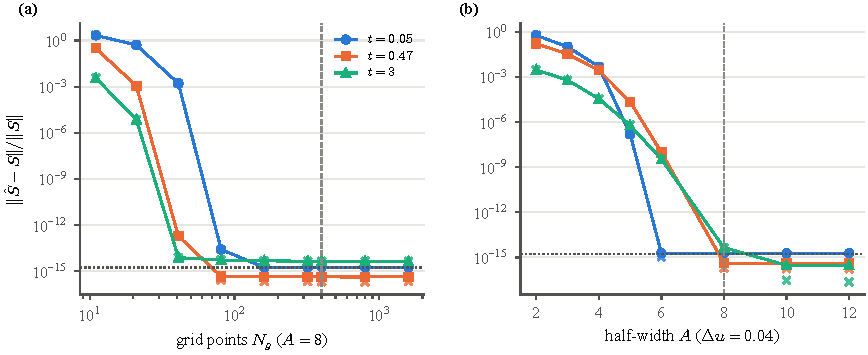
\includegraphics[width=\textwidth]{fig_gaussian_sanity.pdf}
  \caption{\textbf{The Gaussian sanity check (\textsc{e39}).} Pooled relative score error of
  grid BP against the closed-form score (lines) and against an independent
  Kalman--Rauch--Tung--Striebel smoother (crosses) on the Gaussian chain, at the smallest, a
  middle and the largest level. (a) Refining the grid at $\halfwidth=8$; (b) widening the domain
  at the operating spacing. Dashed: the operating grid. Dotted: the smoother against the closed
  form.}
  \label{fig:gaussian}
\end{figure}

Against a finer reference
($\ngrid=1601$, $\halfwidth=12$) the worst relative score error over the twelve levels
and four driving-noise families on ordinary draws is $\gcworstord$; under a
three-standard-deviation displacement the heavy-tailed families lose two orders
(\gcworstshift). The worst forward-message boundary occupancy is $\gcfwdedge$ and the
worst belief edge occupancy $\gcbeledge$ over $\gccells$ production cells.

\paragraph{The envelope, measured rather than inherited.}
\IfFileExists{sections/grid-envelope.tex}{%% Included by A2-numerics.tex only when sections/grid-envelope.tex exists (E11 done).
The validation above fixes the grid at the frozen configuration. Every other
configuration this paper touches---the other driving-noise families, the correlations of
the family ladder, the longer chains of the length study---inherits it, so we measured
it instead: $\gridFamilies$ driving-noise families $\times$ $\gridRhos$ correlations
$\times$ twelve levels $\times$ $\gridSeeds$ seeds, seven candidate grids against a
reference at $\ngrid=\gridRefN$, $\halfwidth=\gridRefA$.

At the frozen configuration the operating grid is comfortable: the pooled drift of the
posterior-mean field is $\gridFrozenDrift$, the worst single level $\gridFrozenDriftWorstLevel$,
and $\gridFrozenBoundary$ of the belief mass lies in the outermost $2\%$ of the domain.
Nothing reported at that configuration is in question.

Over the whole sweep the picture is different, and the difference is instructive: at
half-width $\gridHalfWidth$ the worst-case drift is \emph{flat} in the number of grid
points, $\gridFlatLo$ at $\ngrid=\gridFlatNlo$ and $\gridFlatHi$ at
$\ngrid=\gridFlatNhi$, and falls only when the domain widens---$\gridWiderADrift$ at
$(\gridWiderAN,\gridWiderAA)$ and $\gridWiderBDrift$ at $(\gridWiderBN,\gridWiderBA)$.
That is the signature of truncation rather than of quadrature, and it means refinement
in $\ngrid$ alone, which is what refinement has meant in this literature, cannot fix it.
The binding cell is the $\gridWorstFamily$ family at $\corr=\gridWorstRho$, and the
mechanism is a handful of sites: among the $8192$ sites of each seed's bundle,
$\audExceedCounts$ lie beyond $|a|=\gridHalfWidth$ (the analytic expectation is
$\audExceedExpected$), the largest at $|a|=\audExceedMax$. A site beyond the domain has
its posterior pinned to the boundary on every grid, which is the ``belief mass
$\gridWorstBoundary$ in the outer $2\%$'' of the diagnostic, and at the lowest level its
score error alone is the drift of $\gridWorstDrift$. For a polynomial tail the
expected exceedance count is Poisson with mean $\nseq\nsites\,P(|a|>\halfwidth)$, which no
finite domain makes zero: $\audExceedExpectedTwelve$ per $8192$ sites at
$\halfwidth=12$, $\audExceedExpectedSixteen$ at $\halfwidth=16$. Per replicate of the
family ladder of \cref{app:phase} ($\excChains$ chains of $\excSites$ sites) the same
expectation is $\excStudentRhozeroAeight$ sites at $\halfwidth=8$,
$\excStudentRhozeroAtwelve$ at $12$ and $\excStudentRhozeroAsixteen$ at $16$ for the
Student-$t_5$ chain at $\corr=0$, and below $\excLaplaceRhozeroAeight$ for every other
family and correlation; that ladder therefore quotes the heavy-tailed family from a
recomputation on the $(\phaseWideN,\phaseWideA)$ domain, where its pooled floor has
stopped moving (\textsc{e07b}, \textsc{e07c}); no claim in the body rests on it. The same
consideration governs the closure panel of \cref{fig:theory}: beyond $t\approx3$ the
reference on the $(801,8)$ grid carries the tail of the \emph{truncated} prior, and the
heavy-tailed families depart from the constant for that reason alone; on
$(3201,32)$ they reach it (\cref{app:audit}).

The envelope also has to cover the longer chains of the length study and of the regime
comparison, and it does (\textsc{e11b}: the same sweep at $\nsites\in\{\gridLenList\}$,
$\gridLenSeeds$ seeds). On the operating grid the worst pooled drift over the sweep is
$\gridLenWorstDriftThirtytwo$ at $\nsites=32$, $\gridLenWorstDriftSixtyfour$ at $64$ and
$\gridLenWorstDriftOnetwentyeight$ at $128$, a factor of at most $\gridLenWorstRatioMax$,
and at the frozen configuration $\gridLenFrozenDriftThirtytwo$, $\gridLenFrozenDriftSixtyfour$
and $\gridLenFrozenDriftOnetwentyeight$: the per-site quadrature error does not compound along
the chain, because the messages are renormalised at every site.

A second observation from the same sweep cuts the other way. The column-mass defect of
the discretised kernel, $\max_j|\sum_k \kernel(\gridpt{k}\mid \gridpt{j})w_k-1|$, grows
with correlation, from $\gridColMassLo$ at $\corr=\gridColMassLoRho$ to $\gridColMassHi$
at $\corr=\gridColMassHiRho$, and the reason is again the domain and not the spacing: the
maximum sits in the outermost columns, where a kernel centred at $\corr\gridpt{j}$ with
$|\gridpt{j}|$ near $\halfwidth$ loses the part of its mass beyond the domain, so the
defect is flat in $\ngrid$, falls as the domain widens, and is at machine precision in the
interior columns at every $\corr$. It is not predictive of the error: at
$\corr=\gridColMassHiRho$ the drift is $\gridColMassDriftHiRho$, because the recursion
renormalises every message and the affected columns carry almost no belief. We report it
as a diagnostic and not as an error bar. The uniform family is the one exception to the
quadrature picture: its kernel is discontinuous, the trapezoidal rule is first-order on
it, and its worst-level drift is largest on the coarsest spacing rather than the
narrowest domain.
}{\needsdata{E11 pending: the quadrature envelope across families, correlations and levels}}

\paragraph{Refinement on the reported estimands.}
\IfFileExists{sections/refinement-numbers.tex}{%% Included by A2-numerics.tex only when sections/refinement-numbers.tex exists (E04 done).
Re-scoring the validation-selected kernels of the capacity experiment on their own test
bundles at $\ngrid=801$ and $1601$ ($\halfwidth=8$) and at $\halfwidth=10$
($\ngrid=801$), with the reference recomputed at each resolution, moves the pooled error
of EM--BP ($\ncomp=8$) by at most $\refMoveEmeightDfine\%$, $\refMoveEmeightDfinest\%$
and $\refMoveEmeightDwide\%$ at $\nseq=2048$ (maximum over $\refSeeds$ seeds), and the
LMMSE floor by at most $\refMoveLmmseDfine\%$; the reference score itself moves by
$\refRefMoveDfine\%$ between $\ngrid=401$ and $801$. The reported effects are three
orders of magnitude larger than the discretisation.
}{\needsdata{E04 pending: movement of the headline cells under refinement}}

\paragraph{Floors in the theory verification.}
The outer-product information estimate of a shape coordinate is a small residual of
order-one quantities; for the kinked Laplace density its quadrature floor is reached
near $t=2.5$ at $\ngrid=801$ (the replicate spread stops shrinking), which is why
\cref{fig:theory}b reports the asymptotic slope on the smooth members of the family. The
closure gap of the uniform family reaches the double-precision floor of the BP means
near $t=3.5$, where its squared gap is $10^{-13}$ per chain.
